\iflanguage{ngerman}
{\chapter{Methoden und Umsetzung}}
{\chapter{Methods and Implementation}}
\label{sec:methods}

%design

This chapter describes the layout of the thesis' proposed solution. It also discusses implementation specifics and the tools used to build smart contracts and Jason \ac{BDI} agents. The \ac{BDI} agents are created using the Jason framework and communicate by sending messages and storing the interaction details using Solidity-based smart contracts. We will discuss the application's design objectives and general overview. We will also go through the application's design and functionality for both creating smart contracts independently and after doing so, as well as for creating agents. We discuss the \ac{MAS} and \ac{BCT} implementation specifics, package and library versions utilized, and system configuration. Additionally, the procedures necessary to combine both to contribute to this thesis are also presented. This chapter's prerequisites include understanding the design and architecture of blockchain, AgentSpeak, and \ac{AOP} as described in the previous chapter. The prior chapter's contents should be reviewed to fully comprehend the chapters that follow.

\section{Roadmaps}

The initial roadmap will involve generating multiple agents in a \ac{MAS} and running them simply to see how they fulfill their objectives. Goals are the driving force that directs an agent's proactivity, as agents are expected to actively pursue the goals assigned to them without needing to be constantly stimulated. Examine how agents summon each other by sending messages, as well as how they behave and interact with one another. 

\vspace{.5cm}

The next step will be to create smart contracts for each process on a blockchain. Additionally, while creating the contract, select the appropriate language and version. After ensuring that everything is in order, combine \ac{MAS} and \ac{BCT} and try to run the overall program to ensure compatibility.

\section{Design Goals}

The goal of this project is to create an application that combines \ac{MAS} and \ac{BCT}. We used design considerations that guided our architecture to build such an application.
In considering integrating both technologies, we have specific aims in mind. The following design objectives are listed:
\vspace{.5cm}
\begin{itemize}

    \item \textbf{Decentralization} \\ One of the main advantages of using smart contracts and \ac{BDI} agents in supply chain management is that they allow for decentralized decision-making and coordination. The design of the system should aim to enable decentralization.

    \vspace{.5cm}
    
    \item \textbf{Autonomous} \\Autonomy simply implies being able to work autonomously. To fulfill an objective, an autonomous agent will make independent judgments about how to accomplish its given goals; these decisions and subsequently, its actions are within its control and are not influenced by other forces.

    \vspace{.5cm}

    \item \textbf{Transparency} \\ Smart contracts and \ac{BDI} agents are designed to provide transparency in the supply chain. The design of the system should aim to provide transparency of all activities and interactions among agents, allowing all parties to see the flow of goods within the supply chain.

    \vspace{.5cm}
    
    \item \textbf{Efficiency} \\
    Effectiveness strategies improve the functioning of a smart contract or lower the expenses connected with its use. These patterns can help operators and consumers save time and money.
    
    \vspace{.5cm}

    \item \textbf{Interoperability} \\ The design of the system should aim for interoperability with other blockchain and non-blockchain platforms in order to enable the integration of existing systems and the exchange of information among different platforms.

    \vspace{.5cm}
    
    \item \textbf{Flexibility} \\
    Supply chains are complex and dynamic systems. The design of the system should be flexible enough to adapt to changing conditions in the supply chain. This can be achieved by programming the agents to reason and decide based on their beliefs, desires and intentions which can change over time.
    
    \vspace{.5cm}
    
    \item \textbf{Goal-directed behaviour} \\
    If an agent has been assigned a specific objective, it is assumed that the agent would attempt to attain the goal. Proactivity eliminates completely passive actors who never strive to accomplish anything.

    \vspace{.5cm}
    
    \item \textbf{Reactiveness} \\
    Implementing an application that achieves an appropriate mix of goal-directed and reactive behavior becomes difficult. This is one of the primary design goals of AgentSpeak.
    
    \vspace{.5cm}
    
    \item \textbf{Security} \\
    As \ac{MAS} on the blockchain will handle sensitive information, the security of the system is crucial. The design of the system should aim to protect agents and transactions from malicious actors.

    \vspace{.5cm}
    
    \item \textbf{Scalability} \\ As the number of agents and transactions in a supply chain increases, the scalability of the system can become a challenge. The design of the system should aim for scalability solutions that enable large-scale deployment of agent-based systems on the blockchain.
\end{itemize}

\section{System Configuration And Model Description}

The application is designed to be as basic as possible in order to learn how a supply chain works in the real world, i.e. each entity interacts with the other entity on a different level in order to complete the chain.

    \begin{figure}[h]
    \centering
      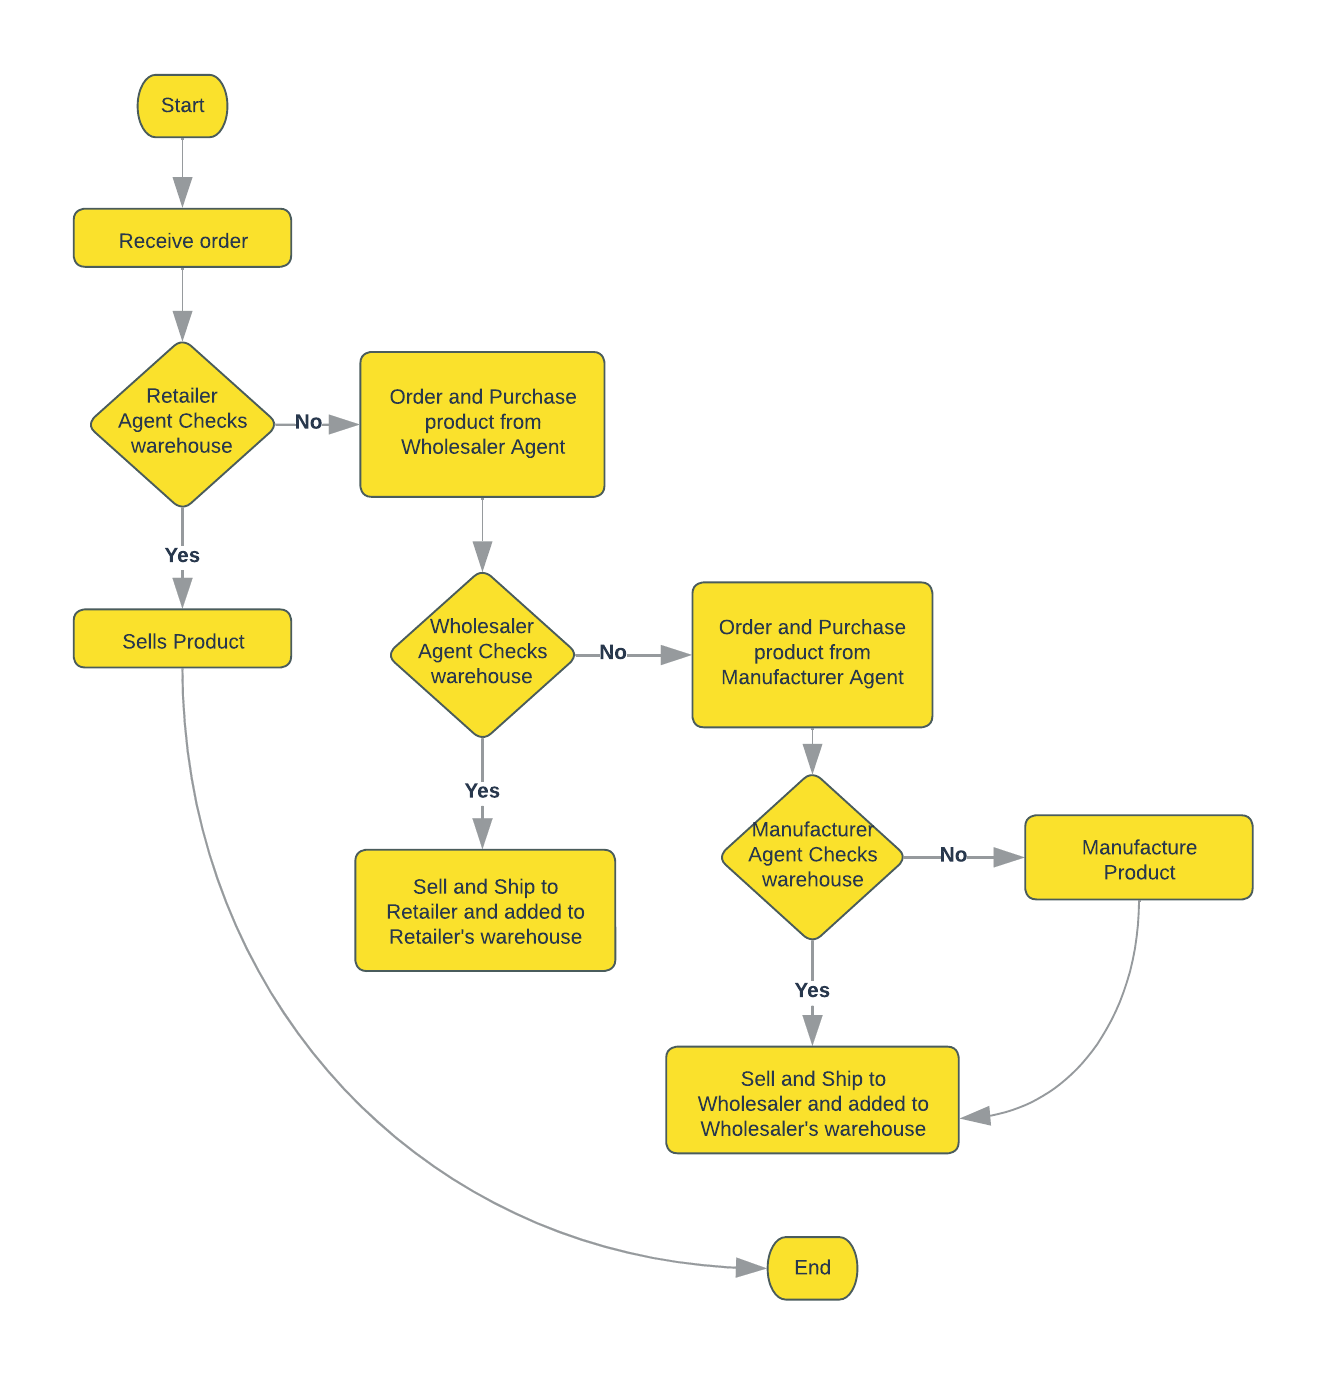
\includegraphics[width=10cm]{includes/figures/Flow Chart.png}
      \caption{Supply Chain Flow Chart}
      \label{Flow chart}
    \end{figure}

\vspace{.5cm}

The application flow for the \textit{Smart contract development with Jason \ac{BDI} agents} is depicted in figure \ref{Flow chart}. These three agents, \texttt{manufacturerAgent}, \texttt{wholesalerAgent}, and \texttt{retailerAgent}, each perform a specific function in the supply chain. All three of the other agents are being invoked by another primary agent i.e., \texttt{mainAgent} in the \ac{MAS}. Figure 
 \ref{Smart Contract Sequence Diagram}  shows the sequence of generating the smart contracts within the supply chain.
Later, figure \ref{Agents in MAS} and \ref{agentsequence} shows the agent interaction, and figure \ref{Sequence Diagram for BDI agents and Smart Contracts} shows the integration of \ac{BDI} agents and smart contracts together.

\vspace{.5cm}

The application was created and tested on a Linux Ubuntu 22.04.1 LTS system.
Visual Studio and InetlliJ are the \ac{IDE} used to create the application. \textit{jEdit} is also used somehow to run agents using Jason framework while creating \texttt{.asl} and running \texttt{.mas2j} file.
To test the compatibility of web3j with gradle for agents, many versions of Java Standard Edition Development Kit were utilized, however the most commonly used was Java SE Development Kit 18.0.2.1. 

\vspace{.5cm}

Other standards for the development of Smart contracts and \ac{BDI} agents are detailed in the sections below.

\section{Smart Contracts Development }   

While taking into consideration the scenario of a supply chain where all information on suppliers, recipients, products, and business circumstances are dispersed over supply chain databases.
It is possible to execute the sale of products or services as a transaction that is cryptographically signed by the seller and the buyer and attached to a smart contract for sales transactions. When the sale occurs and all other conditions, such as documentation and quality checks, are met, the execution of the transfer of the corresponding funds and rights can be enforced; in other words, smart contracts can ensure that collaborative and entrepreneurial processes are carried out correctly.

\vspace{.5cm}

As aforementioned, the terminology blockchain refers to two things: a distributed database and a data structure (i.e. a linked list of blocks containing transactions as shown in figure \ref{Blocks chained together in a blockchain}, where each block is cryptographically chained to the preceding one by incorporating their hash value and a cryptographic signature, in such a manner that changing an earlier block requires re-creating the whole chain since that block). The blockchain technology is connected to the concept of smart contracts, which are scripts that run every time a certain type of transaction occurs and can read and write to the blockchain. Smart contracts allow parties to enforce the requirement that additional transactions occur concurrently with one transaction.

\vspace{.5cm}

    \begin{figure}[h!]
    \centering
      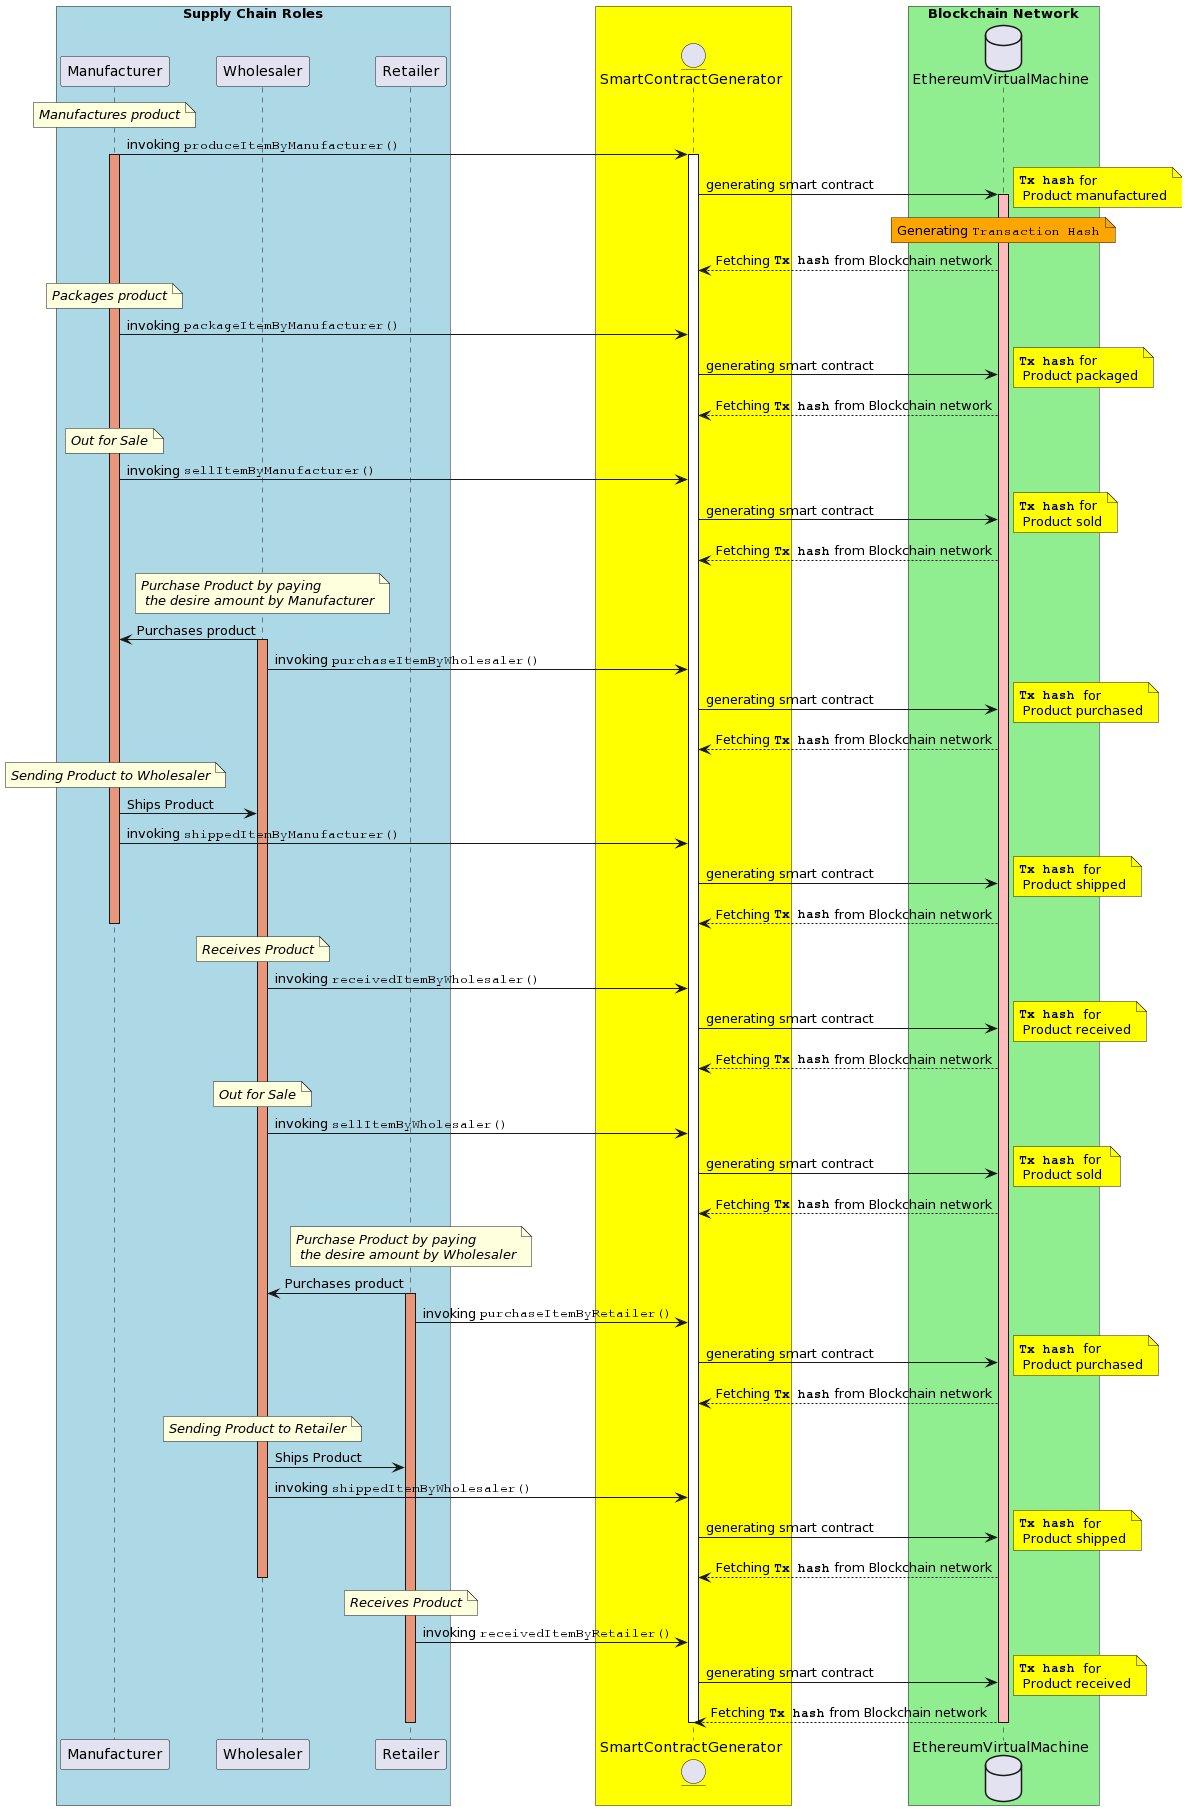
\includegraphics[width=12cm]{includes/figures/Sequence Diagram.png} 
      \caption{Smart Contract Sequence Diagram}
      \label{Smart Contract Sequence Diagram}
    \end{figure}

The programming for smart contracts related supply chain is done while keeping the version in mind in order to integrate it with the agent programming language so that they can work together. Smart contracts perform the following functions with reference to figure \ref{Smart Contract Sequence Diagram}: (1) The product is produced by the manufacturer, (2) the manufacturer completes the packaging, (3) the product is placed on the market, (4) the wholesaler purchases the product, (5) the manufacturer ships the product, (6) the wholesaler receives the product, (7) the wholesaler places the product on the market, (8) the retailer purchases the product, (9) the wholesaler ships the product, and (10) the retailer receives the product as the final result.

\vspace{.5cm}

Each function is regarded as an event, and every event is given a state. It has always been a rule that each event must occur after the one before it has concluded. For example, a manufacturer cannot sell a product before producing it, while a wholesaler cannot receive a product before buying it. It is carried out with the aid of a state check. A product can also be tracked using the \ac{UPC} or by utilizing the \ac{SKU} to trace the entire batch. Later, while integrating smart contracts with agents, the state element was removed to make the supply chain adaptive because there can be sometimes a scenarios when a manufacturer, wholesaler or both will be not a part of the particular supply chain due to the availability of sufficient inventory. Scenarios pertaining to these possibilities are added in the subsequent chapter as a result.

\vspace{.5cm}

Solidity language is used to create smart contracts, while JavaScript is used for testing. The \texttt{.sol} files were compiled using Solidity v0.8.13, to retrieve \texttt{.abi} and \texttt{.bin} files for further implementation and deployment. The truffle tool, especially truffle v5.6.5, has been used for deployment and testing. We have used ganache v7.5.0 and ganache-UI v2.5.4 to examine state and manage chain behavior. All of the packages listed below have been obtained using node v14.0.0 (npm v6.14.4) in the table \ref{Package Version}.

We have used Truffle Suite for the implementation of Solidity-based smart contracts, especially truffle and Ganache. As a programming environment, testing framework, and asset pipeline for blockchains running on the \ac{EVM}, truffle aims to simplify the workload of a developer. Truffle offers built-in binary management, deployment, linking, compilation, and testing for smart contracts in addition to automated contract testing for quick development. It offers a configurable build pipeline with support for tight integration, as well as NPM package management using \ac{NPM} and the ERC190 standard, i.e. \ac{ERC}.

\vspace{.5cm}

Truffle supports transactions and deployments with MetaMask to safeguard your mnemonic, which is a pattern of letters, and it offers enhanced debugging with breakpoints, variable analysis, and step functionality.
With an interactive terminal for direct contract communication, it is an external script runner that runs scripts inside the Truffle environment. Provides a scriptable, extendable framework for deployment and migrations, as well as network management for deploying to any number of public and private networks. Ganache is a private blockchain enabling the speedy production of Corda and Ethereum-distributed applications. Ganache may be used throughout the whole development cycle, allowing you to create, distribute, and test \ac{Dapp} in a secure and predictable setting.

\vspace{.5cm}

Both a \ac{UI} and a \ac{CLI} are available with ganache. A desktop program called Ganache \ac{UI} supports both Corda and Ethereum. Ethereum programming is possible using the powerful command-line tool ganache. It supports snapshot/revert state, Ethereum JSON-RPC compatibility, Zero-config Mainnet and testnet forking, console-log in Solidity, and the ability to impersonate any account without the need for private keys.

\begin{table}[h]
\small
\centering
\caption{Package Version}
\label{Package Version}
\resizebox{5.5cm}{!}{%
\begin{tabular}{|l|l|}
\hline
\textbf{Node Package} & \textbf{Version} \\ 
\hline\hline
web3 & 1.7.5\\ \hline
truffle & 5.6.5\\ \hline 
@truffle/contract & 4.5.22\\ \hline 
@truffle/hdwallet-provider & 2.0.13\\ \hline
dotenv & 16.0.1\\ \hline
geth & 0.4.0\\ \hline
openzeppelin & 4.7.3\\ \hline
\hline 
\end{tabular}}
\end{table}

\vspace{.5cm}

Figure \ref{Activity Diagram} was used as a reference for developing smart contracts connected to the supply chain. The following events were included in the supply chain: To complete the supply chain, (i) the manufacturer manufactures the product, (ii) the manufacturer packages the product, (iii) the manufacturer sells the product to the wholesaler, (iv) the wholesaler purchases the product, (v) the wholesaler receives the product, (vi) the wholesaler sells the product to the retailer, (vii) the retailer purchases the product, (viii) the retailer receives the product and restocks his/her inventory. These events are also covered earlier in this chapter.

\begin{figure}[h]
\centering
  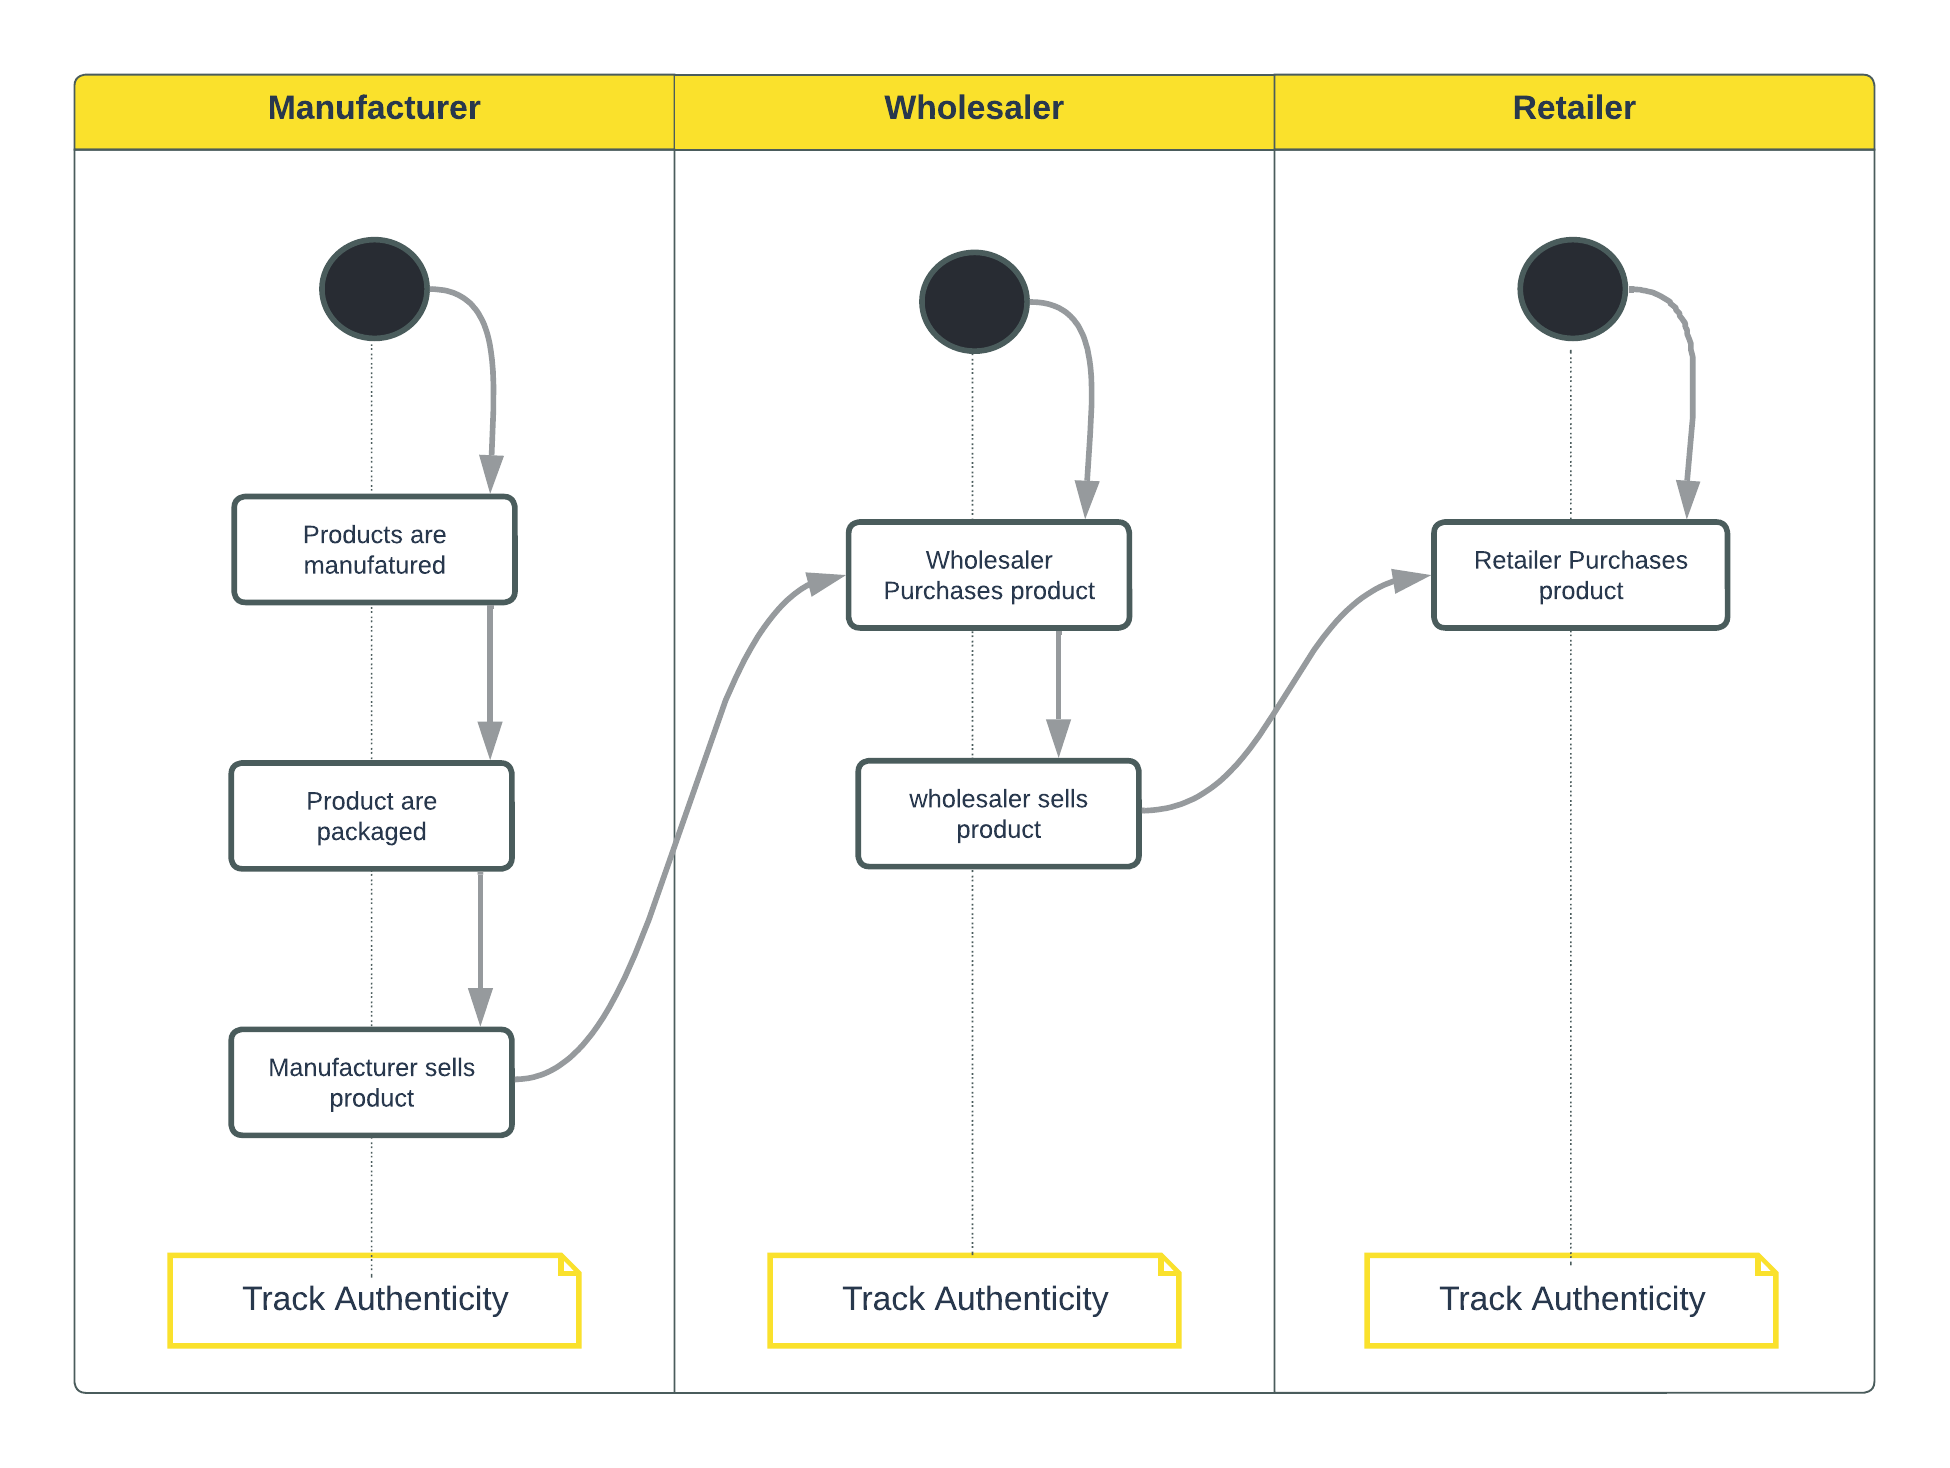
\includegraphics[width=12cm]{includes/figures/Activity Diagram.png} 
  \caption{Supply Chain Activity Diagram}
  \label{Activity Diagram}
\end{figure}

\vspace{.5cm}

To understand the model of the application for smart contracts and the files organized and classes imported using inheritance in-depth, figure \ref{Overall Class Diagram} should be taken into consideration. Solidity contracts can make use of a particular type of format to give detailed documentation for functions, return variables, and other features. The name of this unique format is the \ac{NatSpec}. The formatting for comments used by the author of a smart contract and recognized by the Solidity compiler is included in \ac{NatSpec}\footnote{Check more about NatSpec : https://docs.soliditylang.org/en/v0.8.17/natspec-format.html}. Additionally, third-party tool annotations can be also included in \ac{NatSpec}. The \texttt{@custom:<name>} tag is most likely how they are completed, and analysis and verification tools are an excellent example of this in usage.

\vspace{.5cm}

Aside from Solidity, there are several more languages available for building smart contracts. Vyper was also chosen to construct smart contracts, which is now one of \ac{DeFi}'s most popular languages. Vyper is a high-level programming language identical to Python. However, due to its limitations over Solidity, the proposal was subsequently abandoned.

\begin{figure}[h!]
\centering
  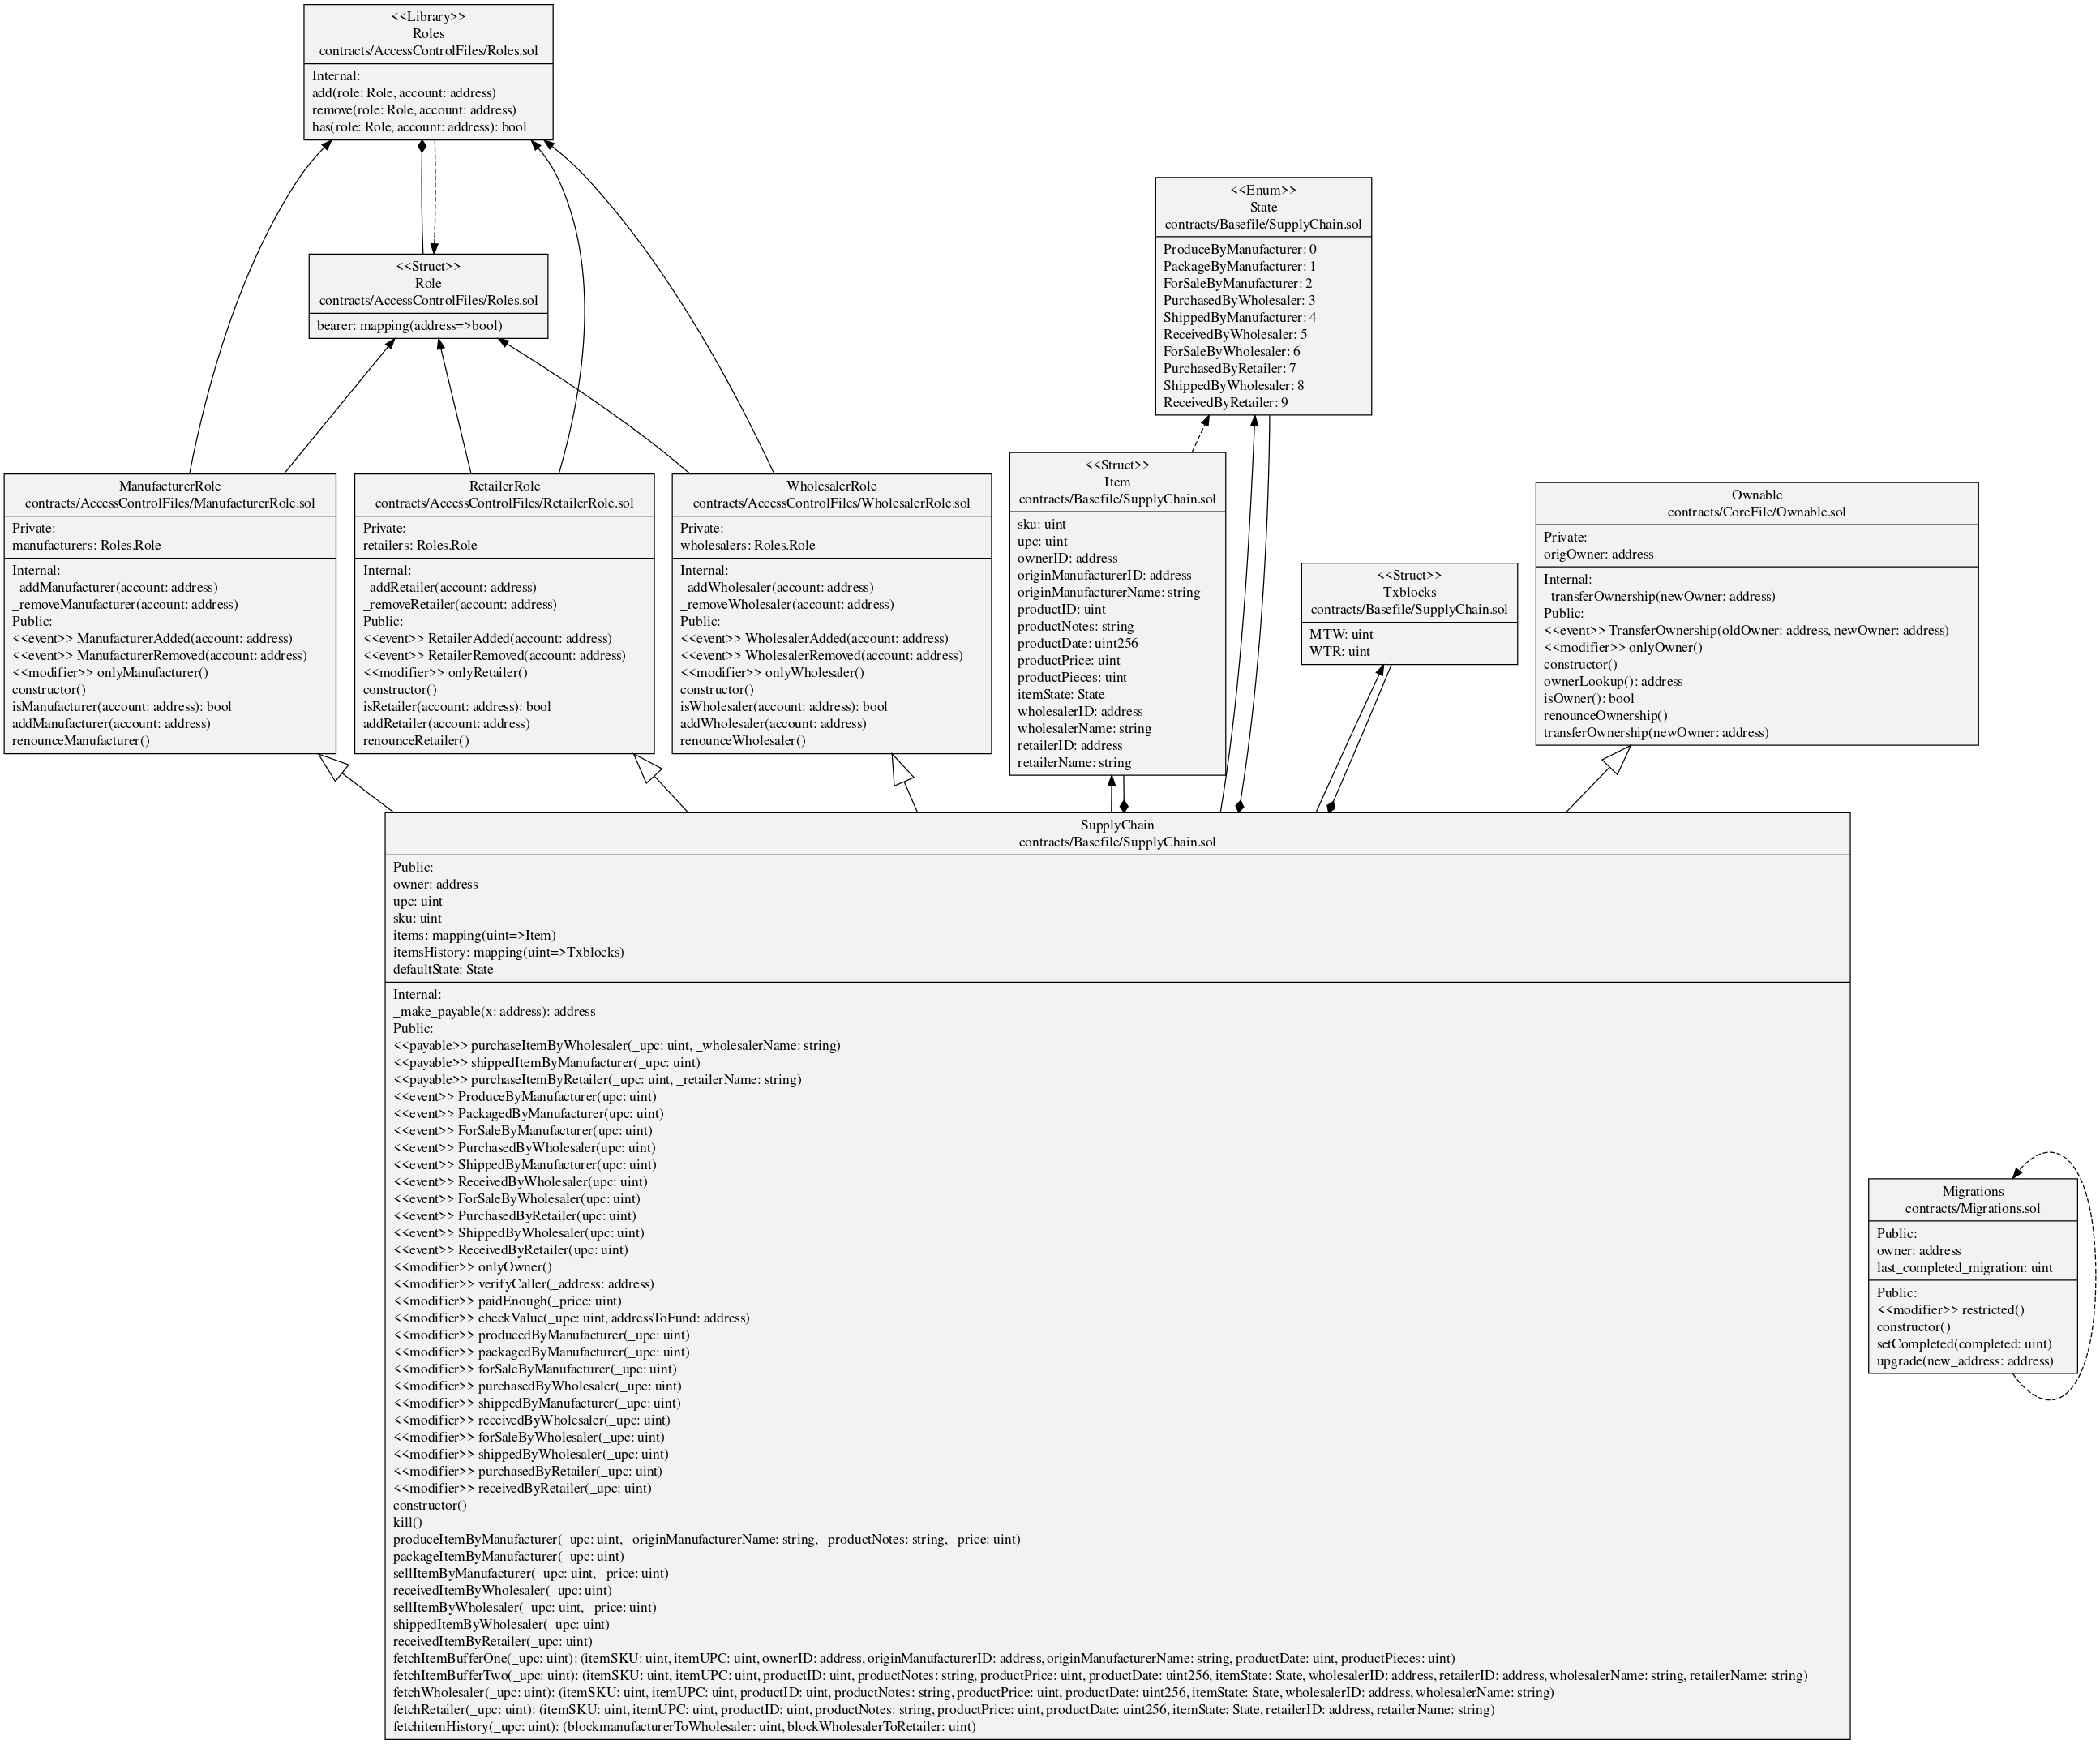
\includegraphics[width=21cm, angle=90]{includes/figures/OverallClassDiagram.png} 
  \caption{Smart Contract Class Diagram}
  \label{Overall Class Diagram}
\end{figure}

\section{Agent Model Implementation}

An agent continually perceives its environment, makes decisions about how to act to achieve its objectives, and then takes action to alter the surroundings. The speech-act theory is commonly used to describe agent communication in \ac{MAS}. The speech-act hypothesis is based on the premise that language is action. An agent program is run by the Jason framework. An agent uses a reasoning cycle to carry out its operations, which may be broken down into the following steps: first, it perceives the environment; second, it updates the belief base; third, it receives communication from other agents; fourth, it selects "socially acceptable" messages; fifth, it chooses an event; sixth, it retrieves all relevant plans; seventh, it determines the applicable plans; eighth, it chooses one applicable plan; and last, it executes one step of an intention.

\begin{figure}[h!]
    \centering
      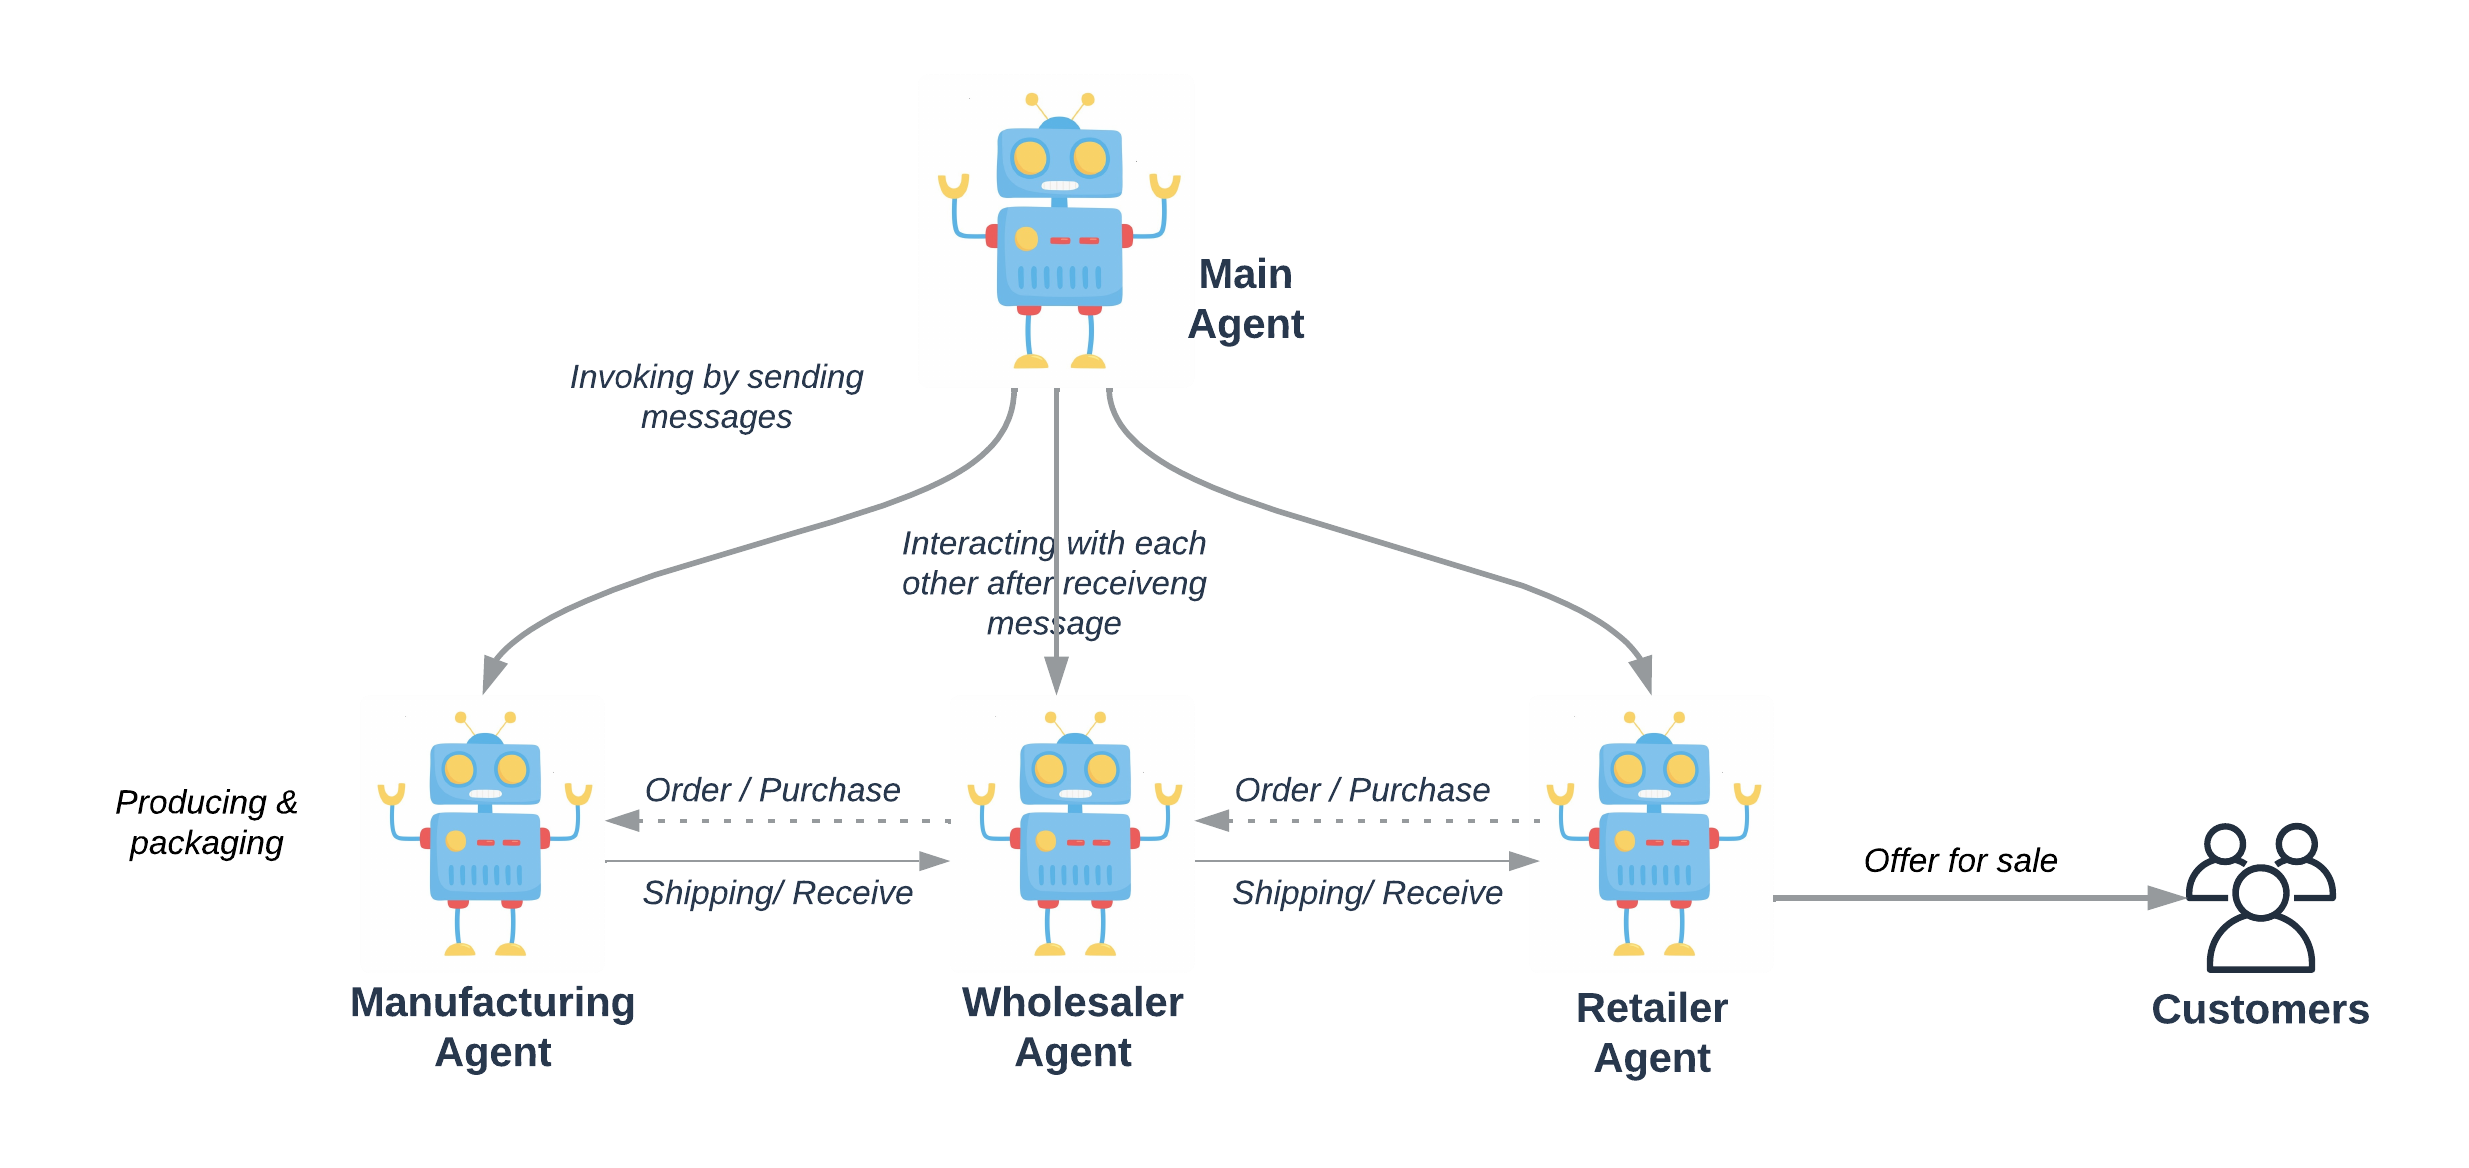
\includegraphics[width=\linewidth]{includes/figures/agent.png} 
      \caption{Agent Interaction in Supply chain}
      \label{Agent Interaction}
    \end{figure}
  
\vspace{.5cm}

In our \ac{MAS}, each agent within the supply chain will act autonomously , see figure \ref{Agent Interaction} to get an idea of how the agents are communicating according to their beliefs, updating them, and executing plans. The \texttt{retailerAgent} will work to ensure that the product is available in the warehouse before ordering it from the \texttt{wholesalerAgent}, who will then ask the \texttt{wholesalerAgent} to check its inventory and if insufficient stock then, get in touch with the \texttt{manufacturerAgent} to produce the product, and ship it to the \texttt{wholesalerAgent}, who will then send it to the \texttt{retailerAgent}. The quantity of stock available and the quantity ordered will be set as belief for each agents as '\texttt{inventory(A).}' and '\texttt{order(B).}', respectively and it will be compared while checking the warehouse before selling product. There will be a \texttt{mainAgent}, who will launch the retailer agent's efforts to sell items to consumers and also other agents by sending messages.

\vspace{.5cm}

The \ac{BDI} architecture is the most common technique to implementing "intelligent" or "rational" agents. The specification of a set of base beliefs and a set of plans results in the creation of an AgentSpeak(L) agent. AgentSpeak(L) differentiates between two kinds of goals: achievement goals and test goals. However, we use achievement targets for our agents. We employed a variety of techniques while writing our agents and ensuring that they could be utilized with smart contracts, and put them appropriately as actions within the suitable plans. We tested several framework with different interpreters and wrote our agents using those. We pursue the following strategies:
 \vspace{.3cm }

\begin{itemize}
    \item \textbf{Jason (Java-based interpreter)}
    \vspace{.3cm }
    \item \textbf{ASTRA}
    \vspace{.3cm }
    \item \textbf{Jason (Python-based interpreter)}

\end{itemize}

The solutions listed above have been defined later in this chapter.

\vspace{.5cm }

\begin{figure}[h]
\centering
  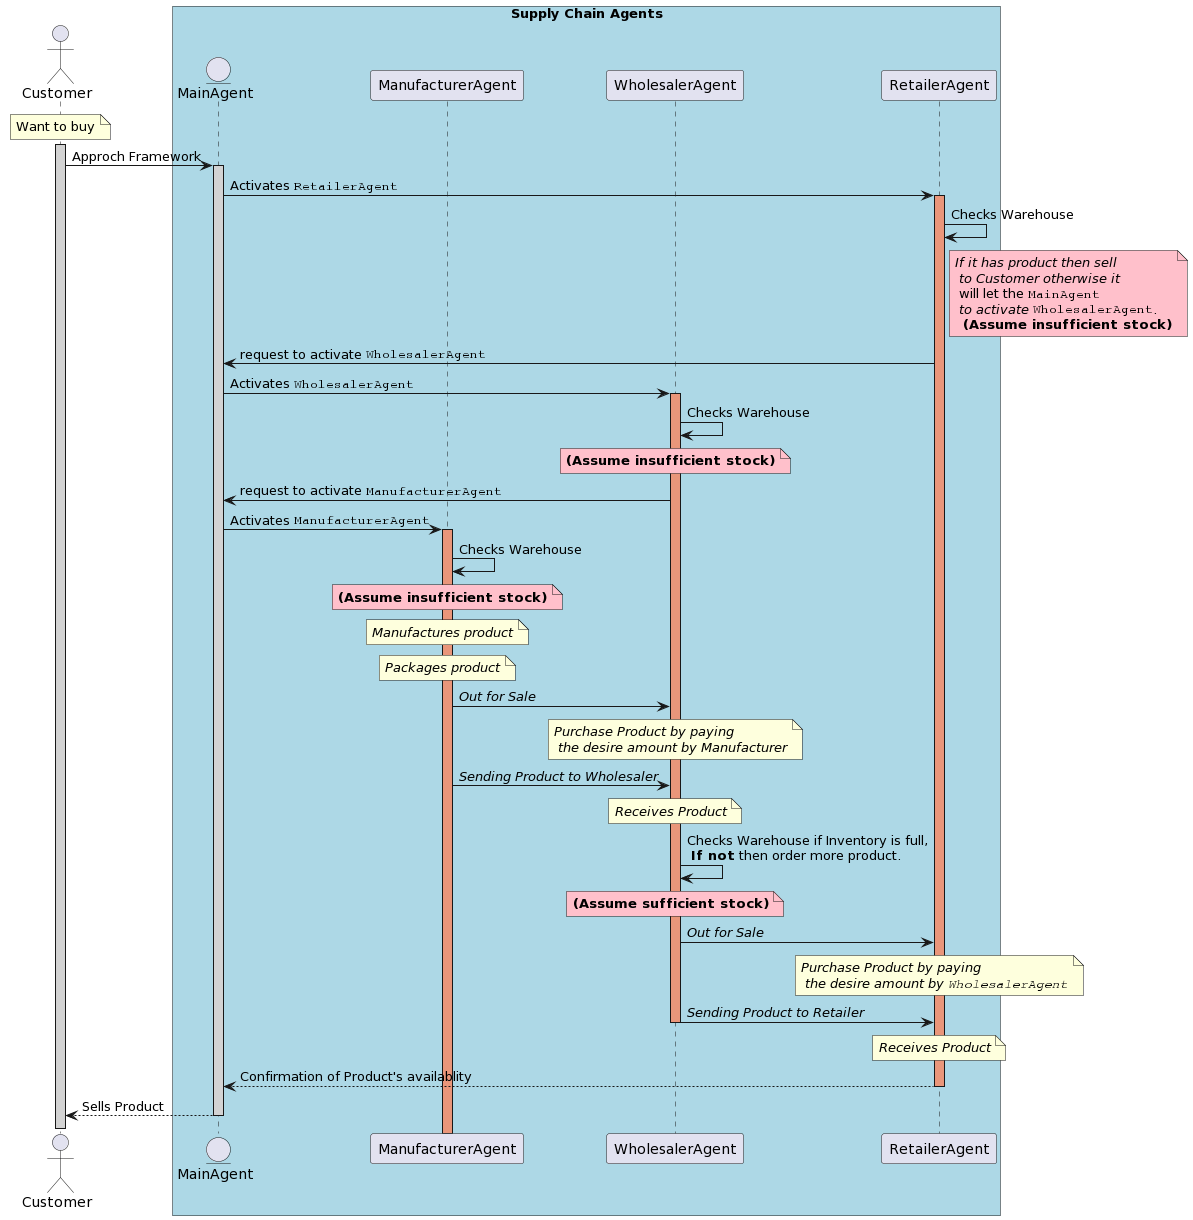
\includegraphics[width=13cm]{includes/figures/agentsequence.png} 
  \caption{Agent Sequence Diagram}
  \label{agentsequence}
\end{figure}

\vspace{.5cm }

The structure of the agent program is governed by the fact that there will be four agents in the \ac{MAS}, as shown in figure \ref{Agents in MAS} in MAS, and they will interact with each other as shown in figure \ref{Agent Interaction}. The sequence of their proper interaction is shown in figure \ref{agentsequence}. Our implementation strategy is as follows:

\begin{itemize}
    \item The supply chain will be initiated by the main agent, who will then engage the retailer agent;
    
    \vspace{.5cm}
    
    \item \texttt{retailerAgent} will inspect its inventory and sell products to customers; if a product is not in stock, \texttt{retailerAgent} will ask the \texttt{mainAgent} to contact the \texttt{wholesalerAgent};
    
    \vspace{.5cm}
    
    \item The \texttt{wholesalerAgent} will check its warehouse and ship the product to the \texttt{retailerAgent}; if the product is not available, the \texttt{wholesalerAgent} will request that the \texttt{manufacturerAgent} be contacted by the \texttt{mainAgent};
    
    \vspace{.5cm}
    
    \item Upon checking its inventory, the \texttt{manufacturerAgent} will ship the product to the \texttt{wholesalerAgent}. If the product is not in stock, the \texttt{manufacturerAgent} will manufacture the product, does the package and deliver it to the \texttt{wholesalerAgent}.

    \vspace{.5cm}
    
    \item \texttt{WholesalerAgent} will strive to keep its inventory full so that it does not have to order every time, therefore it will check its warehouse and order more if it is not full.
    
    \vspace{.5cm}
    
\end{itemize}

Every implementation uses the same approach to how agents cooperate and communicate, and each implementation is elaborated in more detail in the section below.

\begin{figure}[h]
\centering
  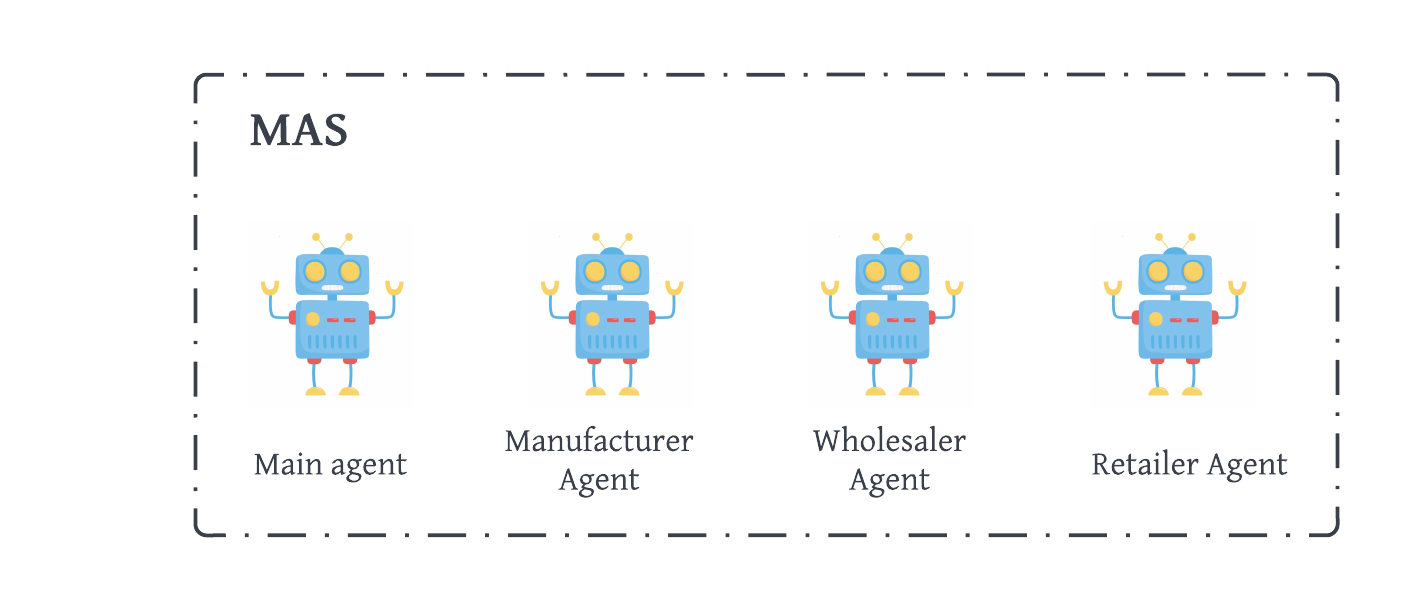
\includegraphics[width=11cm]{includes/figures/MAS.png} 
  \caption{Agents in \ac{MAS}}
  \label{Agents in MAS}
\end{figure}

\subsubsection{Jason (Java-based interpreter)}

We first used Jason with a Java-based interpreter to develop the agents in \ac{MAS}. We set up the home variables, downloaded the necessary scripts and libraries, then used gradle as well as maven for simple configuration. AgentSpeak's expanded dialect has an interpreter named Jason. It implements the operational semantics of that language and offers a platform for creating \ac{MAS} with a variety of characteristics that may be altered by the user. Version 3.1 of Jason, which is the most recent version, was installed. The agents are constructed using figure  \ref{Agent Interaction} as a guide.

\vspace{.5cm}

In addition to being able to interpret the original AgentSpeak, Jason possesses a few other crucial abilities. Inter-agent communication based on speech acts and strong negation are included, allowing for the use of both closed- and open-world assumptions. Additionally, it supports creating environments (which are not normally to be programmed in AgentSpeak; in this case they are programmed in Java). It offers the ability to deploy distributed \ac{MAS} via a network (using \ac{JADE}); the user may also add other distribution infrastructures. Furthermore, it offers an \ac{IDE} in the form of an Eclipse or jEdit plugin; the \ac{IDE} has a "mind inspector" that aids with debugging.

\subsubsection{ASTRA Implementation}

ASTRA programs are divided into agent classes, which may be expanded using a multiple inheritance paradigm. Each agent class is written in a separate file with the same name as the agent class and the \texttt{.astra} extension. ASTRA is distinct from AgentSpeak(L) because ASTRA applications can refer to Java classes, support for delivering fully qualified class names is required. ASTRA programs incorporate partial plans (called plan bodies) in addition to plan rules to promote code/class resuability. ASTRA strives to be familiar to developers who are familiar with mainstream programming languages, particularly Java.

 \vspace{.5cm}
 
Agent Programming Languages are intended to aid in the creation of \ac{MAS}, systems are intended to have more than one agent and more than one agent type by default. Support for deploying numerous agents is given in many Agent Programming Languages via deployment files, which let the developer to define the initial community of agents to be deployed. ASTRA does not support this; instead, you construct an agent that generates new agents. The System \ac{API} provides the essential functionality to allow this approach. In ASTRA, coding one agent to produce another agent is extremely straightforward. You just invoke the System \ac{API}'s \texttt{createAgent(...)} operation.

\subsubsection{Jason (Python-based interpreter)}

An interpreter for Jason, an agent-oriented programming language, built on Python. It can be installed in the system using \texttt{\ac{pip}}. For our implementation, we utilized agentspeak 0.1.0. Python-agentspeak Jason framework is similar to Jason framework with Java, except you don't need to create a \texttt{.mas2j} file to construct a multi-agent system; instead, all the agents may be called together by calling them in a \texttt{.py} file as shown in figure \ref{Agents in MAS}.


\section{Agent-Contract Collaboration}


 We are largely focused on agent-oriented models and technology, and we have smart contracts directly incorporated into the blockchain. With reference to the illustration \ref{Agent Interaction}, the model will be the same for the agents, but their communication will take place via smart contracts, be recorded as transactions on the blockchain, and be subsequently verified using the transaction hashes.

 \vspace{.5cm}
The application flow is developed in accordance with figure \ref{Sequence Diagram for BDI agents and Smart Contracts}, which is an extension of figure \ref{Smart Contract Sequence Diagram} and figure \ref{agentsequence}.

 \begin{figure}[h!]
\centering
  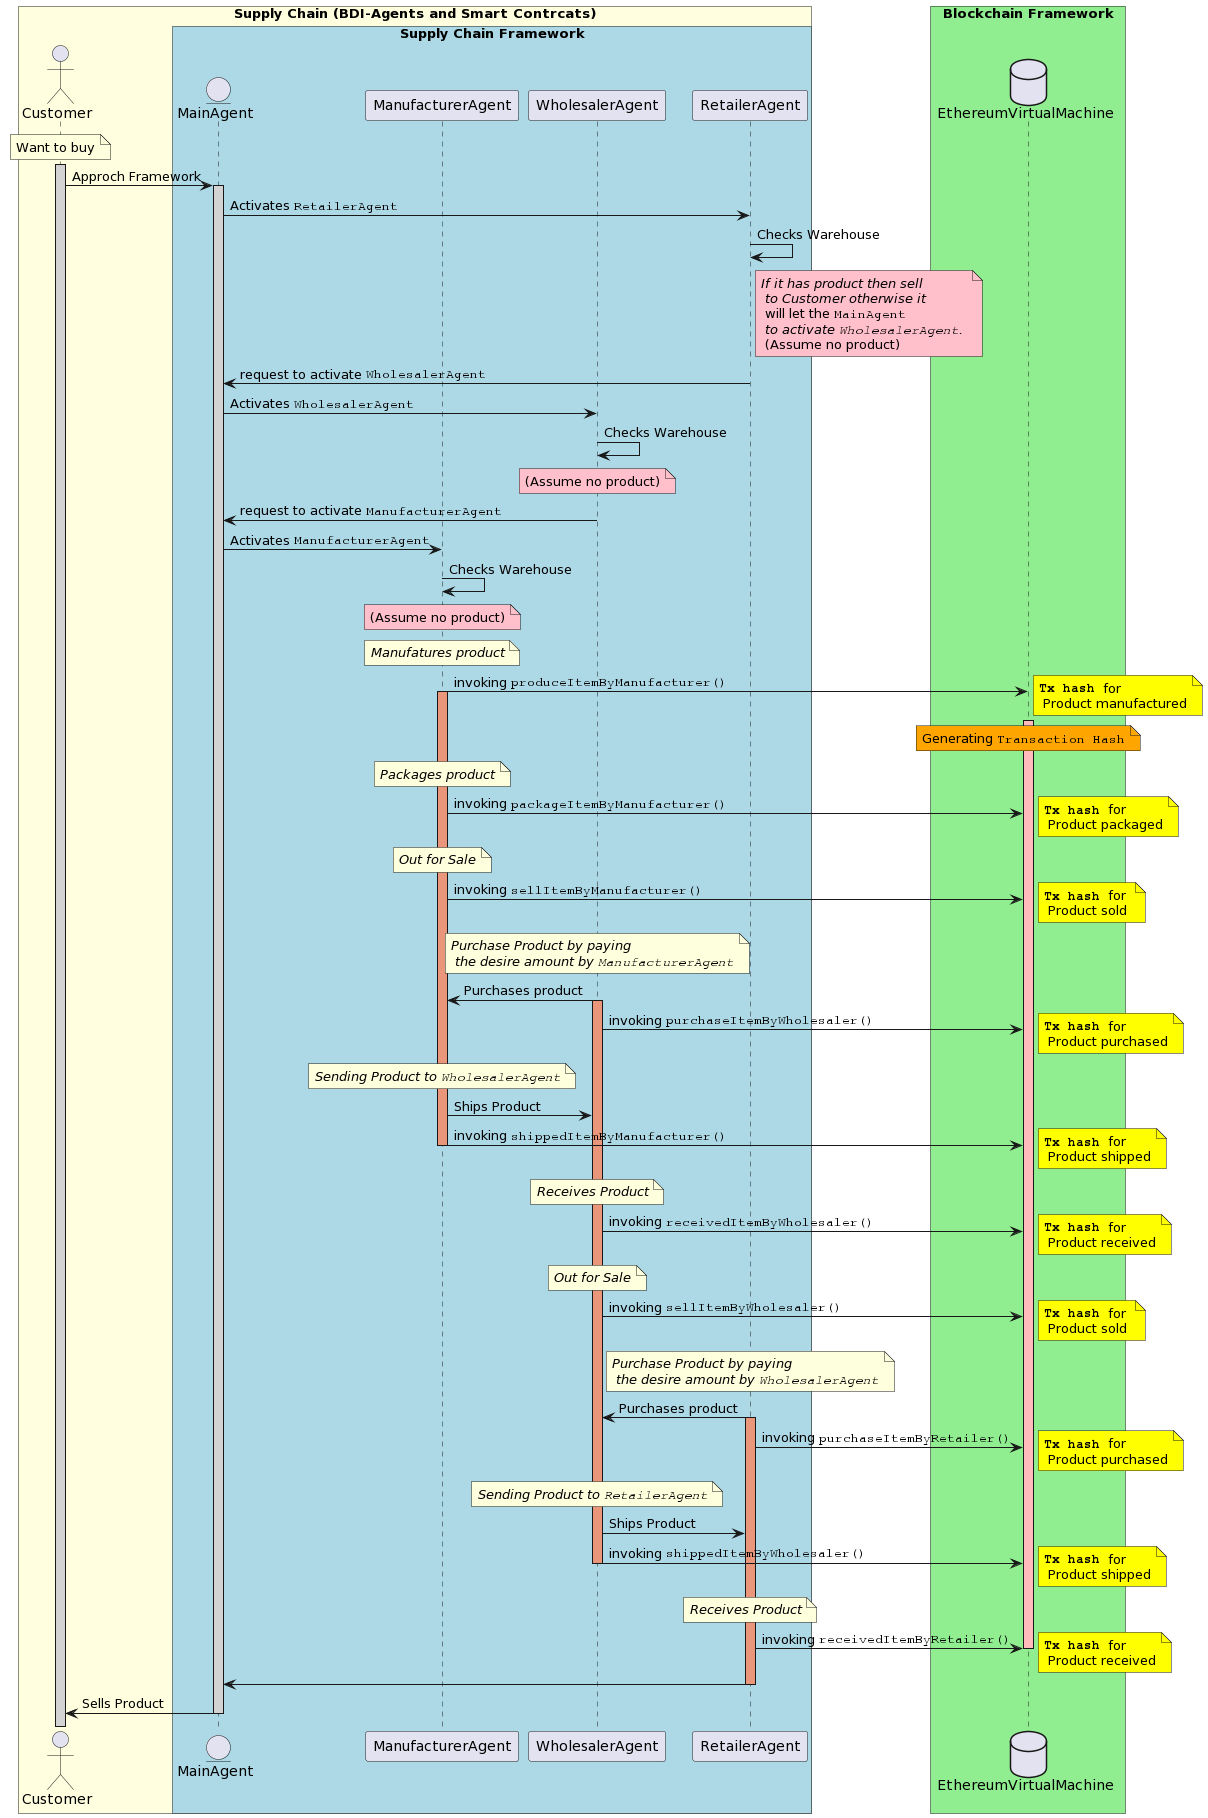
\includegraphics[width=15cm]{includes/figures/sqdgm.png} 
  \caption{Sequence Diagram for \ac{BDI} agents and Smart Contracts}
  \label{Sequence Diagram for BDI agents and Smart Contracts}
\end{figure}

 \vspace{.5cm}

The thesis' core premise is the integration of the two technologies, \ac{MAS} and \ac{BCT}. We have tried to integrate both the technologies using several tries by using several web3 libraries, i.e., \textit{web3.js} for JavaScript, \textit{web3.py} for Python and \textit{web3j} for Java in order to interact with Ethereum. The attempt of linking each framework with each web3 library is detailed below.

\subsubsection{Jason and Web3j}

We attempted to test each smart contract using web3js after generating them with Solidity. We considered migrating to web3j since it would be simpler as opposed to continuing to utilize Jason framework, which is based on Java. Through the command line tools, Web3j facilitates the development of Java smart contract function wrappers from Solidity \texttt{ABI} files or straight from Truffle's contract schema. To reveal the contract's per-network deployment address, a wrapper can be produced. When the wrapper is created, these addresses are from the truffle deployment.

\vspace{.5cm}

The plan to utilize Web3j with Jason was eventually scrapped since, in order for Jason to run \ac{MAS}, the \texttt{.mas2j} file had to be executed, and when it did, it couldn't find the \texttt{org.web3j} package. We attempted to download the jar files locally, change the version of web3j and Jason, and switched from gradle to maven in order to make the program run, but the problem persisted.

\subsubsection{ASTRA and Web3j}

After several attempts with web3j and Jason, we considered switching to ASTRA, a programming language that is quite similar to Java and aims to be familiar to developers with language. A successful agent construction was followed by the same problem as with Jason framework when importing the web3j package.

\subsubsection{Jason and Web3.py}

Web3.py is a Python package that allows you to connect with Ethereum. It is often used in \ac{Dapp}s to support a number of use cases, including sending transactions, communicating with smart contracts, accessing block data, and more. The Web3.js JavaScript \ac{API} served as the foundation for the original \ac{API}, which has since expanded to meet the demands and conveniences of Python developers.

\vspace{.5cm}

The following listing \ref{Web3 library use} demonstrate how to utilize smart contracts with previously deployed contract addresses and link to the Web3 library.

\vspace{.5cm}

\begin{lstlisting}[caption={Web3 library usage},label={Web3 library use},frame=none, numbers=none]
    from web3 import Web3
    web3 = Web3(Web3.HTTPProvider(ganache_url))
    contract_address = web3.toChecksumAddress("0xc9f78D73aCAf603Fe2319682316268A39Cc5CBB7")
    contract = web3.eth.contract(address=contract_address, abi=abi)
    print(f'Deployed Contract Address: {contract.address}')
\end{lstlisting}

\vspace{.5cm}

The code snippet below within the listing \ref{Action defining} demonstrates how to define a specific action regarding product manufacturing i.e., \texttt{produceItemByManufacturer} and store the action in blockchain network when performed by the agent. \ac{BDI} agents created using the Jason framework are capable of performing a variety of actions, and it is also possible to create the custom actions that help us to integrate the smart contract functions with the agents.

\vspace{.5cm}

\begin{lstlisting}[caption={Action defining},label={Action defining}, frame=none, numbers=none]
    actions = agentspeak.Actions(agentspeak.stdlib.actions)
    @actions.add_function(".produceItemByManufacturer", (int, ))
    def produceItemByManufacturer(upc): 
        tx1 = contract.functions.produceItemByManufacturer(upc, "manufacturer_name", "product", 10).transact({
             'from': manufacturer_id
            })
        tx_receipt = web3.eth.wait_for_transaction_receipt(tx1)
        hash = tx_receipt.transactionHash.hex()
        return hash
\end{lstlisting}

\vspace{.5cm}

The code sample below within the listing \ref{Calling action in .asl} demonstrates how specific agents' \texttt{.asl} files can call the functions specified in the actions declared for those agents in the main file to execute a plan and accomplish goals.

\vspace{.5cm}

\begin{lstlisting}[caption={Calling action in .asl},label={Calling action in .asl},frame=none, numbers=none]
    +!manufacture: true
    <-  .print("Manufacturing Product");
        .produceItemByManufacturer(upc, X);
        .print("Tx produceItemByManufacturer successful with hash:", X);
        !package;
        .wait(1000).
\end{lstlisting}

\vspace{.5cm}
\subsubsection{Finale Outcome}

We tested the code several times to make sure it was running correctly by looking at the \texttt{contract address} and \texttt{transaction hashes} from ganache as we were deploying using local network, and each try was successful, as can be seen in the output from one of the evaluations below.

\vspace{.5cm}

Also, regarding the quantity of stock in the warehouse and the batch order for the product, there are several scenarios that might occur as shown in figure \ref{Agent Interaction} and figure \ref{agentsequence}. The results of each scenario are displayed below:

\vspace{.5cm}

\begin{itemize}
    \item Retailer's warehouse has sufficient product, so \texttt{RetailerAgent} doesn't need to order from \texttt{WholesalerAgent}. Listing \ref{Scenario1} below shows the output for the explained scenario.

    \vspace{.5cm}
    \begin{lstlisting}[caption={Agent Interaction (Scenario 1)},label={Scenario1}, numbers=none, basicstyle=\ttfamily\tiny]
    
    <---------------------SMART CONTRACTS AND AGENTS----------------------->
    Deployed Contract Address: 0xc9f78D73aCAf603Fe2319682316268A39Cc5CBB7
    Owner Address: accounts[0] 0xad0BC114B5CF3F0797346fF1Fb1Daf1Cf5123395
    Manufacturer Address: accounts[1] 0x4A9fe326Edc88F1f22940DC9F70BD391fB4218f8
    Wholesaler Address: accounts[2] 0x5fB0Cd136C7A19E8E12F062548002B4460B0dC0d
    Retailer Address: accounts[3] 0xc7D1C50D87B82E85b959DBC2cD9959bfc0480A5E
    <------------------------------------------------------------------------>
    
    <---------------------INTERACTION BETWEEN AGENTS-------------------->
    mainAgent           : Starting SupplyChain with SmartContracts
    mainAgent           : Hi, I am the owner of Contract, with account: 0xad0BC114B5CF3F0797346fF1Fb1Daf1Cf5123395
    mainAgent           : Creating RetailerAgent
    retailerAgent       : Hi, I am here, with account: 0xc7D1C50D87B82E85b959DBC2cD9959bfc0480A5E
    retailerAgent       : Checking Warehouse, and no need to order
    retailerAgent       : Giving products to supplyChainAgent
    mainAgent           : Selling to customers
    mainAgent           : SUPPLYCHAIN COMPLETE
    \end{lstlisting}
    
    \vspace{.5cm}
    
    \item Retailer's warehouse has insufficient product, so \texttt{RetailerAgent} need to order from \texttt{WholesalerAgent} and Wholesaler's warehouse has sufficient product, so \texttt{WholesalerAgent} doesn't need to order from \texttt{ManufactureAgent}. Listing \ref{Scenario2} below shows the output for the explained scenario.

    \vspace{.5cm}
    \begin{lstlisting}[caption={Agent Interaction (Scenario 2},label={Scenario2},numbers=none, basicstyle=\ttfamily\tiny]
    <---------------------SMART CONTRACTS AND AGENTS----------------------->
    Deployed Contract Address: 0xc9f78D73aCAf603Fe2319682316268A39Cc5CBB7
    Owner Address: accounts[0] 0xad0BC114B5CF3F0797346fF1Fb1Daf1Cf5123395
    Manufacturer Address: accounts[1] 0x4A9fe326Edc88F1f22940DC9F70BD391fB4218f8
    Wholesaler Address: accounts[2] 0x5fB0Cd136C7A19E8E12F062548002B4460B0dC0d
    Retailer Address: accounts[3] 0xc7D1C50D87B82E85b959DBC2cD9959bfc0480A5E
    <------------------------------------------------------------------------>
    
    <---------------------INTERACTION BETWEEN AGENTS-------------------->
    mainAgent           : Starting SupplyChain with SmartContracts
    mainAgent           : Hi, I am the owner of Contract, with account: 0xad0BC114B5CF3F0797346fF1Fb1Daf1Cf5123395
    mainAgent           : Creating RetailerAgent
    retailerAgent       : Hi, I am here, with account: 0xc7D1C50D87B82E85b959DBC2cD9959bfc0480A5E
    retailerAgent       : Checking Warehouse
    retailerAgent       : INSUFFICIENT INVENTORY!! Ordering Product..
    retailerAgent       : Ordering to wholesalerAgent
    mainAgent           : Creating WholesalerAgent
    wholesalerAgent     : Hi, I am here, with account: 0x5fB0Cd136C7A19E8E12F062548002B4460B0dC0d
    wholesalerAgent     : Checking Warehouse, and no need to order
    wholesalerAgent     : Selling product to retailerAgent
    wholesalerAgent     : Tx sellItemByWholesaler successful with hash: 0x421c5ed80a71376a4e8e4e7b6a4083bd8e83f734ed43c67130847eab0f2c7fdf
    retailerAgent       : Purchasing product from wholesalerAgent
    retailerAgent       : Tx purchaseItemByRetailer successful with hash: 0xc07aba5f53bb5d74ce1aea3d788d0c65cb34a036a1459750e9d2db6d9e81cda0
    wholesalerAgent     : Shipping product to retailerAgent
    wholesalerAgent     : Tx shippedItemByWholesaler successful with hash: 0x33e0b25c8d44b837b573ed00e1fe34315c6de613fcacfa2856a4f1cb10671be3
    retailerAgent       : Received product from wholesalerAgent and Inventory full!!
    retailerAgent       : Tx receivedItemByRetailer successful with hash: 0xcc84c9fe3cd74b803419e4dde53f71f0d01243ea0d4ec1873b5aadb95cba23e2
    retailerAgent       : Checking Warehouse, and no need to order
    retailerAgent       : Giving products to supplyChainAgent
    mainAgent           : Selling to customers
    mainAgent           : SUPPLYCHAIN COMPLETE
    \end{lstlisting}
    
    \vspace{.5cm}

    \item Retailer's warehouse has insufficient product, so \texttt{RetailerAgent} need to order from \texttt{WholesalerAgent}, Wholesaler's warehouse has also insufficient product, so \texttt{WholesalerAgent} need to order from \texttt{ManufactureAgent} and Manufacture's warehouse has sufficient product, so \texttt{ManufactureAgent} doesn't need to manufacture product. Listing \ref{Scenario3} below shows the output for the explained scenario.

    \vspace{.5cm}
    \begin{lstlisting}[caption={Agent Interaction (Scenario 3},label={Scenario3}, numbers=none, basicstyle=\ttfamily\tiny]
    <---------------------SMART CONTRACTS AND AGENTS----------------------->
    Deployed Contract Address: 0xc9f78D73aCAf603Fe2319682316268A39Cc5CBB7
    Owner Address: accounts[0] 0xad0BC114B5CF3F0797346fF1Fb1Daf1Cf5123395
    Manufacturer Address: accounts[1] 0x4A9fe326Edc88F1f22940DC9F70BD391fB4218f8
    Wholesaler Address: accounts[2] 0x5fB0Cd136C7A19E8E12F062548002B4460B0dC0d
    Retailer Address: accounts[3] 0xc7D1C50D87B82E85b959DBC2cD9959bfc0480A5E
    <------------------------------------------------------------------------>
    
    <---------------------INTERACTION BETWEEN AGENTS-------------------->
    mainAgent            : Starting SupplyChain with SmartContracts
    mainAgent            : Hi, I am the owner of Contract, with account: 0xad0BC114B5CF3F0797346fF1Fb1Daf1Cf5123395
    mainAgent            : Creating RetailerAgent
    retailerAgent        : Hi, I am here, with account: 0xc7D1C50D87B82E85b959DBC2cD9959bfc0480A5E
    retailerAgent        : Checking Warehouse
    retailerAgent        : INSUFFICIENT INVENTORY!! Ordering Product..
    retailerAgent        : Ordering to wholesalerAgent
    mainAgent            : Creating WholesalerAgent
    wholesalerAgent      : Hi, I am here, with account: 0x5fB0Cd136C7A19E8E12F062548002B4460B0dC0d
    wholesalerAgent      : Checking Warehouse
    wholesalerAgent      : INSUFFICIENT INVENTORY!! Ordering Product..
    wholesalerAgent      : Ordering to manufacturerAgent
    mainAgent            : Creating ManufacturerAgent
    manufacturerAgent    : Hi, I am here, with account: 0x4A9fe326Edc88F1f22940DC9F70BD391fB4218f8
    manufacturerAgent    : Checking Warehouse
    manufacturerAgent    : Quantity alread exist in inventory, dont need to manufacture!
    manufacturerAgent    : Selling product to wholesalerAgent
    manufacturerAgent    : Tx sellItemByManufacturer successful with hash: 0x95c053089529888fb8c399355e666e6827935cc1b3e45b4bce90ccbc07eccd6b
    wholesalerAgent      : Purchasing product from manufacturerAgent
    wholesalerAgent      : Tx purchaseItemByWholesaler successful with hash: 0x28719d94c2f40383a74c25d39859dc4a1f26b06d0adb6d39f5e20ab7a5f6f499
    manufacturerAgent    : Shipping product to wholesalerAgent
    manufacturerAgent    : Tx shippedItemByManufacturer successful with hash: 0x5cbf427497b18c441dc7d44808cfd522c1f62e41a0c7c8524acb63a8aa8b4461
    wholesalerAgent      : Received product from manufacturerAgent, and added to the inventory and Inventory FULL!!
    wholesalerAgent      : Tx receivedItemByWholesaler successful with hash: 0x3ff03e21cd1b42eea4a55504dca701cd16484408acd9831f7f6a5df216f46e2e
    wholesalerAgent      : Checking Warehouse, and no need to order
    wholesalerAgent      : Selling product to retailerAgent
    wholesalerAgent      : Tx sellItemByWholesaler successful with hash: 0x5a786f97f9ff516c319e1473c8fff3b850c68010ea37ea32778f8f53e6704090
    retailerAgent        : Purchasing product from wholesalerAgent
    retailerAgent        : Tx purchaseItemByRetailer successful with hash: 0xb2a75b53a5f4ee86551a6a31d8324fd807376c2bc03a0a6b3d0585f5819be626
    wholesalerAgent      : Shipping product to retailerAgent
    wholesalerAgent      : Tx shippedItemByWholesaler successful with hash: 0x3fc8c3f81c033257ab58c5f9ca09197e7eafe7a61a6df4ba9b60e054ed7fb42a
    retailerAgent        : Received product from wholesalerAgent
    retailerAgent        : Tx receivedItemByRetailer successful with hash: 0x70660ae51b082f39a551e8c0132058c1bbc557267826ecd81ed59006025b5722
    retailerAgent        : Checking Warehouse, and no need to order
    retailerAgent        : Giving products to supplyChainAgent
    mainAgent            : Selling to customers
    mainAgent            : SUPPLYCHAIN COMPLETE
    \end{lstlisting}
    
    \vspace{.5cm}

    \item Retailer's warehouse has insufficient product, so \texttt{RetailerAgent} need to order from \texttt{WholesalerAgent}, Wholesaler's warehouse has also insufficient product, so \texttt{WholesalerAgent} need to order from \texttt{ManufactureAgent} and Manufacture's warehouse has also insufficient product, so \texttt{ManufactureAgent} needs to manufacture product. In this scenario, \texttt{WholesalerAgent} ordered again because it wanted to make its inventory full. Listing \ref{Scenario4} below shows the output for the explained scenario.

    \vspace{.5cm}
    \begin{lstlisting}[caption={Agent Interaction (Scenario 4},label={Scenario4}, numbers=none, basicstyle=\ttfamily\tiny]
    <---------------------SMART CONTRACTS AND AGENTS----------------------->
    Deployed Contract Address: 0xc9f78D73aCAf603Fe2319682316268A39Cc5CBB7
    Owner Address: accounts[0] 0xad0BC114B5CF3F0797346fF1Fb1Daf1Cf5123395
    Manufacturer Address: accounts[1] 0x4A9fe326Edc88F1f22940DC9F70BD391fB4218f8
    Wholesaler Address: accounts[2] 0x5fB0Cd136C7A19E8E12F062548002B4460B0dC0d
    Retailer Address: accounts[3] 0xc7D1C50D87B82E85b959DBC2cD9959bfc0480A5E
    <------------------------------------------------------------------------>
    
    <---------------------INTERACTION BETWEEN AGENTS-------------------->
    mainAgent            : Starting SupplyChain with SmartContracts
    mainAgent            : Hi, I am the owner of Contract, with account: 0xad0BC114B5CF3F0797346fF1Fb1Daf1Cf5123395
    mainAgent            : Creating RetailerAgent
    retailerAgent        : Hi, I am here, with account: 0xc7D1C50D87B82E85b959DBC2cD9959bfc0480A5E
    retailerAgent        : Checking Warehouse
    retailerAgent        : INSUFFICIENT INVENTORY!! Ordering Product..
    retailerAgent        : Ordering to wholesalerAgent
    mainAgent            : Creating WholesalerAgent
    wholesalerAgent      : Hi, I am here, with account: 0x5fB0Cd136C7A19E8E12F062548002B4460B0dC0d
    wholesalerAgent      : Checking Warehouse
    wholesalerAgent      : INSUFFICIENT INVENTORY!! Ordering Product..
    wholesalerAgent      : Ordering to manufacturerAgent
    mainAgent            : Creating ManufacturerAgent
    manufacturerAgent    : Hi, I am here, with account: 0x4A9fe326Edc88F1f22940DC9F70BD391fB4218f8
    manufacturerAgent    : Checking Warehouse
    manufacturerAgent    : INSUFFICIENT INVENTORY!! Manufacturing Product..
    manufacturerAgent    : Tx produceItemByManufacturer successful with hash: 0xde3468f453048739395cfe770a2be70654ac05d7fe006fd77ad2e91e55cd0fb5
    manufacturerAgent    : Packaging Product
    manufacturerAgent    : Tx packageItemByManufacturer successful with hash: 0xac339f4c9d1bd18c206c4fefa2da1578255ab184cfb56a19aa5f0c749691c90f
    manufacturerAgent    : Checking Warehouse
    manufacturerAgent    : Quantity alread exist in inventory, dont need to manufacture!
    manufacturerAgent    : Selling product to wholesalerAgent
    manufacturerAgent    : Tx sellItemByManufacturer successful with hash: 0x70d3e37c5cae73f9e3721dd1cec079b2329f241d035bc3c0d8d5435c9980291a
    wholesalerAgent      : Purchasing product from manufacturerAgent
    wholesalerAgent      : Tx purchaseItemByWholesaler successful with hash: 0x45057874c25a62ad149fc3e984a6856fc8ca3865fe8f1faa558e237b84437a87
    manufacturerAgent    : Shipping product to wholesalerAgent
    manufacturerAgent    : Tx shippedItemByManufacturer successful with hash: 0x9ae2c0454a62266658d252827a852d8c4f2636ce106e5fe122c0a0fce1f49518
    wholesalerAgent      : Received product from manufacturerAgent, and added to the inventory and and Inventory not full yet!!
    wholesalerAgent      : Tx receivedItemByWholesaler successful with hash: 0x7b2b32121504e0c424faf0721aba7dde1152781d8e6ca099146bca2a99321863
    manufacturerAgent    : Selling product to wholesalerAgent Again
    manufacturerAgent    : Tx sellItemByManufacturer successful with hash: 0xb5b7ed54756b9123522d942c131f52a79450ed8a61b5b5f17b5e762c4dfd2c96
    wholesalerAgent      : Purchasing product from manufacturerAgent Again
    wholesalerAgent      : Tx purchaseItemByWholesaler successful with hash: 0x0000ce3707589a17982b27b0efb13872ffc8b2c8ff509e3783f19fa2e81a2263
    manufacturerAgent    : Shipping product to wholesalerAgent
    manufacturerAgent    : Tx shippedItemByManufacturer successful with hash: 0xdc4e1db2675c4a85b20eca1ce2e94ce9064ae8ec4d7160c23f5dc3e682e714b1
    wholesalerAgent      : Received product from manufacturerAgent, and added to the inventory and Inventory FULL!!
    wholesalerAgent      : Tx receivedItemByWholesaler successful with hash: 0x130f6ac86210088f05687b9d769615856bc0da2459c5ff68640330c2e8ffcf66
    wholesalerAgent      : Tx receivedItemByWholesaler successful with hash: 0xe37eb45b7918a377f96daaf95be30432d2c8902f3033c0809fc3a1ec0970bcf5
    wholesalerAgent      : Checking Warehouse, and no need to order
    wholesalerAgent      : Selling product to retailerAgent
    wholesalerAgent      : Tx sellItemByWholesaler successful with hash: 0x6aaf996c1a2347612b38350cc31c20320d25d21da80878be1776cbd1f8138258
    retailerAgent        : Purchasing product from wholesalerAgent
    retailerAgent        : Tx purchaseItemByRetailer successful with hash: 0x18677b7134c6ee338ac749c090e4121f2fa80308837da9f1c8f13955841e411a
    wholesalerAgent      : Shipping product to retailerAgent
    wholesalerAgent      : Tx shippedItemByWholesaler successful with hash: 0x45e406258e946a2eee2969dbf5461c799d036190598677a3b787b3e93bbf9ddd
    retailerAgent        : Received product from wholesalerAgent
    retailerAgent        : Tx receivedItemByRetailer successful with hash: 0x24d53dcdb1b44e2b86938daa9df29ad8efd7f40718a73d0f3a4aff9437c2f68f
    retailerAgent        : Checking Warehouse, and no need to order
    retailerAgent        : Giving products to supplyChainAgent
    mainAgent            : Selling to customers
    mainAgent            : SUPPLYCHAIN COMPLETE
    \end{lstlisting}
    
    \end{itemize}


The output above demonstrates how the various supply chain roles interact with one another to complete the process of planning, manufacturing, and delivering a product or service. It demonstrates that each role has been given an \texttt{account number} and that whenever they interact or complete a procedure, a \texttt{transaction hash} is issued to verify its authenticity and for future use.

\vspace{.5cm}

Jason's Python interpreter and Web3.py worked well together. In order to communicate or convey messages from one agent to another, \texttt{.asl} files for the each agent were written with belief sets and plans with goals and a \ac{MAS} was produced using Python with AgentSpeak as shown in figure \ref{Agents in MAS}, which is a bit different from Jason constructed using Java. Additionally, running a \texttt{.mas2j} file is not necessary for \ac{MAS} in Jason-style AgentSpeak for Python.

\subsubsection{Jason and Jython}

Jython is a Python programming language implementation meant to operate on the Java platform. JPython was the previous name for the implementation. Any Java class may be imported and used by Jython apps. With the exception of a few common modules Jython applications employ Java classes rather than Python modules. 

\vspace{.5cm}
Jython provides practically all of the modules found in the standard Python programming language package, with the exception of a few modules written in C. Jython either dynamically or statically converts Python source code to Java bytecode (an intermediate language). The following tasks are especially well suited for Jython:

\begin{itemize}
    \item In order to interact with Java packages or run Java programs, Jython provides an interactive interpreter. This makes it possible for developers to experiment with and debug any Java system using Jython.
    \vspace{.5cm}
    \item Users can write simple or intricate scripts using embedded scripting to increase an application's capabilities. The Jython libraries are available to Java programmers for their systems.
    \vspace{.5cm}
     \item Python scripts are frequently 2–10 times shorter than their Java equivalents, enabling quick development of applications. This has a direct impact on how efficiently programmers work. Python and Java get along well with one another, allowing programmers to mix the two languages at will during both product development and release.
\end{itemize}

\vspace{.5cm}

Jason AgentSpeak's smart contract development for Python and Web3.py was a success, so we decided to give it another shot and try to develop it using Jython. The Jython project provides Python implementations in Java, giving Python the benefits of operating on the JVM and access to Java classes. We remained adamant about running it in Java and used the \texttt{web3j} package to integrate \ac{BCT} into \ac{MAS}. We attempted to use Jason with Java by converting the Python code into a Java application. The creation of a Java application containing Python code was successful, but when the \texttt{.mas2j} file was executed, but it was unable to import the package \texttt{org.python}, which is necessary to start the program.

\vspace{.5cm}

The next chapter explains the results from our suggested approaches for taking the steps along smart contracts deployed in a bespoke blockchain with their own flow of control among agents constructed utilizing agent oriented language.

